\chapter{Background}


\section{Breast Cancer}

A study in Sweden by \textcite{tabar2001} found breast carcinoma mortality was reduced by 63\% after mammography was introduced. This clearly emphasize the benefits of screening which has resulted in an increased usage of this method to detect and diagnose breast cancer. The increasing demand for mammography image interpretation has lead to a shortage of medical radiologist to perform this task, consequently non medical personnel supplement the mammography image interpretation \parencite{culpan2016}. As breast cancer still continues to be the leading cause of cancer mortality among women and more efficient diagnostics and pathology is high on demand, the need of low-cost point-of-care is very large \parencite{martei2018}.

Fine needle aspiration (FNA) is a diagnostic tool to aspirate cell samples by sampling cells from a tumour, then staining them, and examine under a microscope \parencite{FNA}. An example of such sample can be seen in figure \ref{fig:fna_nuclei}. The cell samples can be evaluated within 24 hours and the method is cost-effective and can be used as a preoperative tool for investigation of tumours. The method is also complication-free and has been widely used for the past 60 years.

\begin{figure}[ht!]
  \centering
  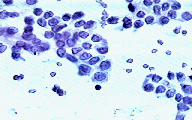
\includegraphics[]{images/fna_nuclei.png}
  \caption[]
  {\small A caption of a FNA sample as seen through a microscope. The sample is collected from a breast lump by fine needle aspiration then stained to engender the features of the cells. Image courtesy of \textcite{dua:2017}.}
  \label{fig:fna_nuclei}
\end{figure}


\section{Computer Aided Diagnostics}

Machine learning techniques have been successfully applied to computer aided diagnostics (CAD). By a computerized procedure it provides a second, objective opinion of medical image interpretation and diagnosis \parencite{li2007}, \parencite{ni2016}. To create a CAD system, samples with a diagnose is firstly gathered and stored, then used for learning. In the case of breast cancer detection, a radiologist put labels on a set of mammography scans. These include the diagnosis of the scan and possibly additional attributes connected to the scan too, such as patients age or other conditions. These scans together with the labels can then be used to learn a hypothesis whether a undiagnosed sample contains benign or malignant cancer \parencite{li2007}.


\section{Machine Learning}

The field of machine learning is concerned with automated discoveries of regularities in data with use of computer algorithms. These regularities can then be used to take actions, such as classifying data into different categories or making predictions \parencite{Bishop:2006}. As the data may differ from images to population growth to medical data, the computer algorithms differ too. The algorithms used in this report is detailed below.

\subsection{Artificial Neural Networks}

The term Artificial Neural Network (ANN) originates from the structure of the algorithm. The structure vaguely mimics the biological network of a human brain \parencite{Bishop:2006}. A representation of such network is visualized in figure \ref{fig:ANN_representation}. The learning process of an ANN is conceptually two parts, feed forward and back propagation.

\begin{figure}[ht!]
  \centering
  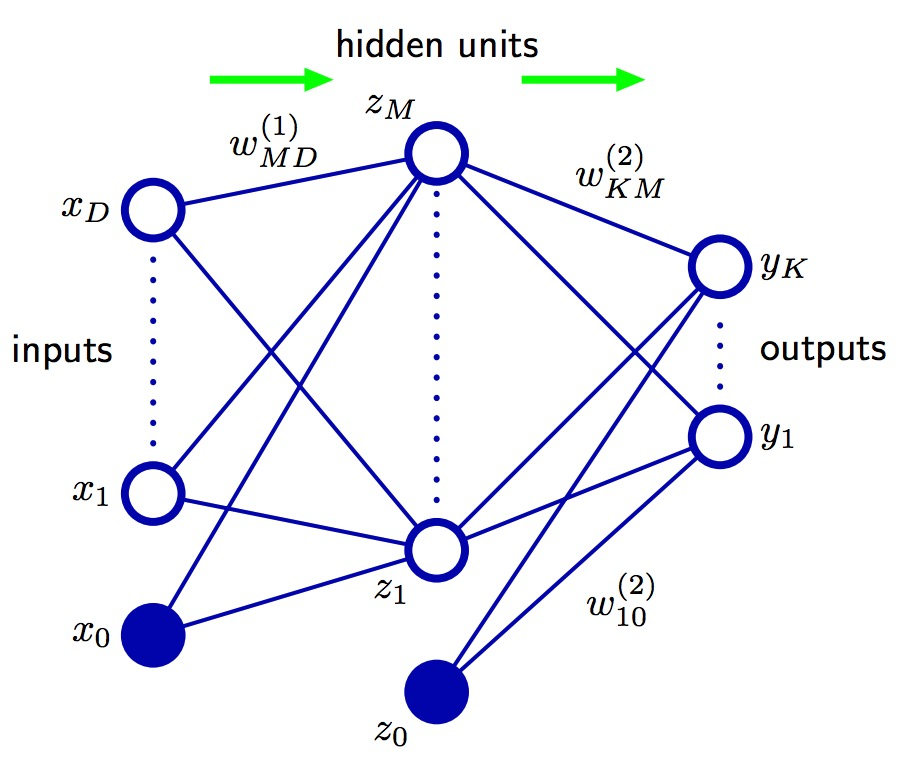
\includegraphics[width=0.7\linewidth]{images/ANN_representation.jpg}
  \caption[]
  {\small Network diagram for a two layer neural network. $X_D$ represents the input data which is linearly transformed by the weights $W_{MD}$ and bias $X_0$ and forwarded to the hidden units. From the hidden units the data is transformed in the same manner to the output layer $y_K$ which corresponds to the potential classes of the input data. Image courtesy of \textcite{Bishop:2006}.}
  \label{fig:ANN_representation}
\end{figure}

% Image found at page 228 in Bishop book: http://users.isr.ist.utl.pt/~wurmd/Livros/school/Bishop%20-%20Pattern%20Recognition%20And%20Machine%20Learning%20-%20Springer%20%202006.pdf

When initially feeding forward the data constitutes the input of the network. The input signal is equal to the dimensionality of the data. Forwarding the signal to the first layer, a linear transformation is applied to the signal involving two parameters conclusive to the layer, weight and bias. The transformed signal is sent through an activation function amplifying or reducing the signal based on its current value, producing a new output. This output is then considered the input for a new set of weights and biases, then forwarding the signal repeatedly in the same manner until reaching the final layer. In the final layer the signal is converted to probabilities, one for each possible output of the network \parencite{Bishop:2006}.

Back propagation is where an ANN is tuning its wights and biases to produce sensible outputs in relation to the input. Feeding an input of training data forward, an error can be computed from the difference between the received output probabilities and the expected output. The error is in turn propagated backwards, tuning the parameters to produce the expected output instead. Repeating this process for all training data the network can increase its prediction accuracy by tuning itself to the data \parencite{Bishop:2006}.

\subsection{Decision Trees}

Tree based methods involve stratifying or segmenting the predictor space into a number of simple regions. In order to make a prediction for a given observation, the mean or the mode of the training observations is used in the region to which it belongs. Since the set of splitting rules used
to segment the predictor space can be summarised in a tree, these types of approaches are known as Decision Trees (DT) \parencite{James:2014}.

DTs can be applied both to regression as well as classification problems. We focus on classification DTs as its the nature of the classification at hand in this report.

To grow a classification tree recursive
binary splitting is performed. The binary spilt is based on classification error rate on the training data. Since we want the classifier to assign an observation in a given region to the most commonly occurring error rate class of training observations in that region. The classification error rate is simply the fraction of the training observations in that region that do not belong to the most common class \parencite{James:2014}.

\subsection{Naïve Bayes}

Naïve Bayes (NB) have beens studied since the 1950s and is a supervised, probabilistic machine learning classifier. It uses the posterior which statistically determines the probability of a data point $x$ belonging to a certain class $y$ given the observed data points:

\[
P(y|x) = \frac{P(x|y)P(y)}{P(x)}
\]

This formula can be read as:

\[
Posterior = \frac{Prior * Likelihood}{Evidence}
\]

Where Prior is the prior probability of $y$ belonging to some distribution $\theta$, likelihood the probability of $x$ belonging to distribution $\theta$ when having observed $y$. The evidence is the probability of $\theta$, and finally the Posterior is the conditional probability of $y$ given $x$. The name of the methods originates from the fact that the maximum posterior is calculated with help of the Bayes' Theorem and the method is naïve in the aspect of it assuming that all features in the data are independent form each other \parencite{george2012}.


\subsection{Support Vector Machines}

Support vector machines (SVM) were developed in the 1990s and are based on the simpler maximal margin classifier. The maximal margin classifier creates a hyperplane to separate the data points of different classes from each other. The margin is the smallest perpendicular distance from the plane to a data point. As the name of the method suggests, the goal is to find the plane with the largest margin given the data set \parencite{James:2014}.

\begin{figure}[ht!]
  \centering
  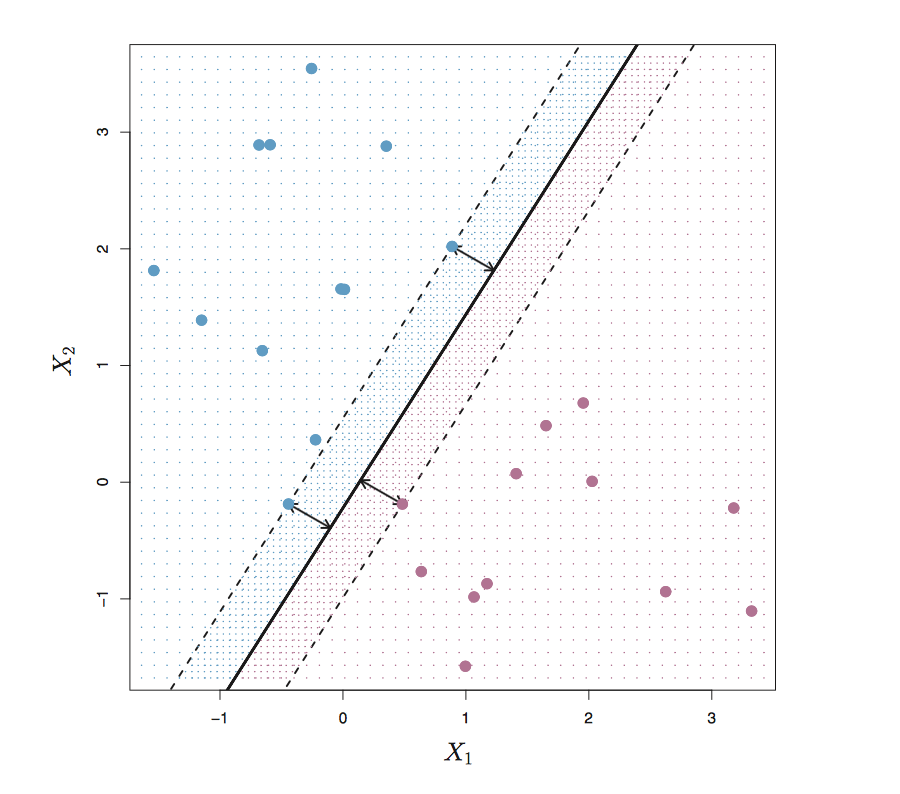
\includegraphics[width=0.7\linewidth]{images/Margin_SVM.png}
  \caption[]
  {\small Image of SVM margin. The red dots represent one class and the blue dots represent another class. The arrows indicates the maximal margin. Image courtesy of \textcite{James:2014}.}
  \label{fig:SVM_Margin}
\end{figure}

The support vector classifier is an extension to the maximal margin method to try create a method with greater robustness and better classification to most training observations. In order to achieve this goal, a slack variable in introduced to allow points to be on the wrong side of the margin. Lastly, a SVM converts the support vector classifier from a liner separator to a non-linear separator by using so called Kernels. The classifier can now separate more complex data sets with higher accuracy since its not limited to create linear hyperplanes \parencite{James:2014}.


\section{Feature Selection}

A feature is a variable that describes a data instance. A rectangular surface can be considered having two features, length and height. A rectangular volume can be considered having three features: length, height and depth. More complex data instances, such as a gene expression may have up to $60\,000$ features, such vast feature space results in a much harder learning process. Thus, many times it is preferable to select a subset of all available features to reduce the dimensionality \parencite{guyon2003}.

The benefits of selecting a subset of all available features are manyfold, among other it facilitates data visualization and data understanding. It reduces the measurement and storage requirements and reduces training and utilization times. In cases with thousands of features, like the example with gene expressions, it is essential to work with a subset of the data to produce reliable results \parencite{guyon2003}.


\subsection{Filter Methods}

Filter methods are considered a preprocessing step. That means a filter method evaluate features before data is applied to a learning machine, or even before a deciding on a classifier. The evaluation is performed by doing variable ranking by some score, such as information gain. The score results in a ranking of the attributes and a subset can be selected in order of the ranking \parencite{guyon2003}.

There are both good and bad aspects of filter methods. The positive concerns variable ranking make filter methods very scalable and robust, as the calculations only operates on as many variables as there are features. They can be performed just once and tested on multiple classifiers making it very computational effective. On the other hand, a subset of features that independently might be assessed an non informative, may in combination with other features provide a lot of information to enable good learning \parencite{guyon2003}.


\subsection{Wrapper Methods}

Wrapper methods differs significantly from filter methods. While filter methods are evaluated as a preprocessing step, independent of the classifier, wrapper are evaluated dependent on the classifier.

Wrappers utilize the learning machine of interest as a black box to score subsets of variables according to their predictive power \parencite{guyon2003}. The issue is that as datasets become large this method might be overly computational intense, as finding the optimal subset is considered to be NP-hard \parencite{amaldi1998}.

% Image source: http://webcache.googleusercontent.com/search?q=cache:635J2rrIdWsJ:pages.cs.wisc.edu/~olvi/uwmp/cancer.html+&cd=1&hl=sv&ct=clnk&gl=se

\section{Related Work}

Medical datasets have been widely used to assess the performance of a multitude of classification strategies and methods. Breast cancer is one of the disease commonly studied within the filed of machine learning \parencite{kononenko2001}.

\subsection{Optimization of Classification Accuracy in CAD}

Multiple studies exploring optimal classifiers for CAD have been conducted. \textcite{ramos2012} tested $20\,000$ classifier configurations to evaluate their ability to correctly classify malignant cancer. They achieved a result of 0.996 under the Receiver operating characteristic (ROC) curve. The method to achieve this result was a feed forward, back propagating ANN.

With a foundation of well performing classifiers such as \parencite{ramos2012}, studies investigating more fine tuned approaches building upon earlier results have been made. \textcite{akin2011} demonstrated that ensemble learning can be used in CAD to improve the performance of a rotation forest classifier. Using three different dataset and 30 classifying algorithms the average accuracy improved on all datasets by nearly 3\%.

\textcite{Abdel-Ilah2017} reported further improvements on ANNs by investigating the optimal number of hidden layers and neurons for a feed forward back propagation network on the WBCD dataset which is included in our experiments as well. The highest accuracy achieved was 98\% using 3 hidden layers and 21 neurons with three distinct transfer functions.

\subsection{Optimization Classification Accuracy in CAD using Feature Selection}


There are several ways to optimize a machine learning methodology. \textcite{c201416} explains that feature selection algorithms can be used for a vast amount of benefits such as: simplicity, stability, classification accuracy, storage and computational requirements. They also claim that comparison between different feature selection methods can only be done on one dataset at a time since the underlying algorithms depend on the structure of the data. Improvement in prediction accuracy was achieved in the paper by using feature selection for several datasets to demonstrate the applicability of feature selection techniques.

\textcite{akay2009} investigated the performance of classification of a SVM with a RBF kernel using feature selection, filtering by F-score. They achieved a classification accuracy of 99.51\% which accordingly was among the highest scores recorded by then (2007). It should be noted, the accuracy was measured on only one dataset meaning the result can not be generalized to datasets at large. The dataset was WBCD.

\textcite{b20103177} demonstrated how  binary particle swarm optimization (BPSO) and genetic algorithm (GA) techniques as feature selection methods improved the accuracy for classifying coronary artery disease using a SVM. The feature selection methods only used 11 features and 12 features respectively compared to the full data set of 23 features and achieved an improvement of 2-4\% accuracy.

\textcite{karabulut2012} made a comparative study on the effect of feature selection on classification accuracy and found up to 15.55\% improvement (an increase from 55.56\% to 71.11\%) on classification rates using a ANN classifier. The study used only filter algorithms for feature selection, among those were both information and Chi2. The study applied the selected features on three classification methods, Naïve Bayes, Artificial Neural Network as Multilayer Perceptron, and J48 decision tree classifier on 15 different datasets including WBCD.

Building upon this foundation of work our study seeks to complete the field by providing further investigation of unreported selection methods such as SBS and SFS and review their performance on a combination of classifiers from the previous research presented here.
